\documentclass[11pt]{article}
% Horizontal Magnetic Dipole over a lossy half-space
\usepackage[utf8]{inputenc} % Use it to include other characters than ABC
\usepackage[cmex10]{amsmath}
\usepackage{mdwmath}
\usepackage{mdwtab}
\usepackage{hyperref}
\usepackage{physics} % For using the oridnary derivative nomenclature
\usepackage{datetime} % Insert date and time
\usepackage[letterpaper, margin=1in]{geometry}
\usepackage{graphicx}
% \usepackage{mathptmx} % Times new Roman

% ------------------------------- Useful Tricks Learnt
% Use ={}& to align subequations to the left
% Use = for single equations
% Put comments % in between the lines in order to avoid forming a new paragraph.
% To enter special characters into Inkspace figures, use Ctrl+U and then enter       the unicode. e.g., for \times symbol, the unicode is U+0D7. So the key entry would be Ctrl+U U+0d7 and then press enter.
%
% ----------------- To compile with references use the following order in Shell"
% 1. pdflatex filename.tex
% 2. bibtex filename (no extension)
% 3. bibtex filename (no extension)
% 4. pdflatex filename.tex
% -----------------

% Personal definitions
% Operators
\renewcommand{\v}[1]{\mathbf{#1}} % vectors
\newcommand{\ti}[1]{\tilde{#1}} % spectral representation

% Symbols
\renewcommand{\O}{\omega}  % omega
\newcommand{\E}{\varepsilon}  % epsilon
\renewcommand{\u}{\mu}  % mu
\newcommand{\p}{\rho}  % rho
\newcommand{\x}{\times}  % times
\renewcommand{\inf}{\infty}  % infinity
\newcommand{\infint}{\int\limits_{-\inf}^\inf} % integral by R
\newcommand{\del}{\nabla}  % nabla operator
\renewcommand{\^}{\hat}  % unit vector


\begin{document}
  \title{\textsc{Equivalent Tranmission Line Models for Layered Structures with Sources}\\}
  \date{\footnote{Last Modified: \currenttime, \today.}}
  \maketitle
  We consider a multilayered structure with piece-wise material that is assumed unbounded in the tranverse direction
  \begin{subequations}
    \begin{align}
      \del\x{\v E} ={}& -j \O \u \v{H} -\v{M},
      \label{eq:E}\\
      \del\x{\v H} ={}& j \O \E \v{E} + \v{J}.
      \label{eq:H}
    \end{align}
    \label{eq:MaxE}
  \end{subequations}

  For boundary-value problems involving planarly multilayer structures displaying symmetry along the $z$ direction, it is desirable to decompose the $\v{\del}$ operator into two components, one $\dv{}{z}$ and the other to a transverse (to z) operator, $\v{\del_t}$ \cite[p. 64]{felsen1994radiation}. The analysis can be simplified by taking Fourier transform represented by the operator $\mathcal{F}$, in both $x$ and $y$ directions. This transforms the $\v{\del}$ operator to $-j k_x \v{\^{x}} - j k_y \v{\^{y}} + \v{\^{z}}\dv{}{z}$
  containing only a single derivative in $z$.
  The Fourier transform along with its inverse is defined as:

  \begin{subequations}
    \begin{align}
      \mathcal{F}[f(\v{r})] \equiv \ti{f}(\v{k_{\p}},z) ={}& \infint \infint
      f(\v{r}) \exp(-j \v{k_{\p}} \cdot \v{\p}) dx dy
      \label{eq:Fourier}\\
      \mathcal{F}^{-1}[\ti{f}(\v{k_{\p}},z)] \equiv f(\v{r}) ={}& \frac{1}{(2\pi)^2} \infint \infint \ti{f}(\v{k_{\p}},z)
      \exp(j \v{k_{\p}} \cdot \v{\p}) dk_x dk_y
      \label{eq:IFourier}
    \end{align}
    \label{eq:FT}
  \end{subequations}
  where,
  \begin{equation}
    \v{\p} = x\v{\^{x}} + y\v{\^{y}},
    \v{k_{\p}} = k_x\v{\^{x}} + k_y\v{\^{y}},
  \end{equation}
  and the $~$ above indicates the Fourier transform with respect to the transverse coordinates.

  As stated earlier, it is advantageous to separate the fields in transverse and longitudinal coordinates since as we shall shortly, the longitudinal component can be completely described in terms of the transverse one. Taking the Fourier transform of the Maxwell's equations (\ref{eq:MaxE}), we obtain:

  \begin{subequations}
    \begin{align}
      \left(-j\v{k_{\p}} + \v{\^{z}} \dv{}{z} \right)\x (\v{\ti{E}_t} + \v{\ti{E}_z})  ={}& -j \O \u (\v{\ti{H}_t} + \v{\ti{H}_z}) -
      (\v{\ti{M}_t} + \v{\ti{M}_z}),
      \label{eq:FT_E}\\
      \left(-j\v{k_{\p}} + \v{\^{z}} \dv{}{z} \right)\x (\v{\ti{H}_t} + \v{\ti{H}_z})  ={}& j \O \E (\v{\ti{E}_t} + \v{\ti{E}_z}) -
      (\v{\ti{J}_t} + \v{\ti{J}_z}),
      \label{eq:FT_H}
    \end{align}
    \label{eq:FT_MaxE}
  \end{subequations}

  Separating the transverse and longitudinal components in (\ref{eq:FT_E}), we write:
  %
  \begin{subequations}
    \begin{align}
      -j\v{k_{\p}} \x \v{\ti{E}_z} +
      \dv{}{z}\v{\^{z}} \x \v{\ti{E}_t} ={}&
      -j \O \u \v{\ti{H}_t} -
      \v{\ti{M}_t},
      \label{eq:FT_TE}\\
      -j\v{k_{\p}} \x \v{\ti{E}_t} ={}&
      -j \O \u \v{\ti{H}_z} -
      \v{\ti{M}_z},
      \label{eq:FT_LE}
    \end{align}
    \label{eq:FT_TLE}
  \end{subequations}
  %
  Using the vector cross product property \cite[p. 117]{fang2009antenna},
  \begin{equation}
    \v{A}\x\v{B} =\v{A}\cdot (\v{B} \x \v{\^{n}})\v{\^{n}}
    \label{eq:vec}
  \end{equation}
  %
  where the unit vector $\v{\^{n}}$ is normal to the plane containing vectors $\v{A}$ and $\v{B}$, we obtain a scalar form of the longitudinal component of the electric field. Applying the aforementioned property on (\ref{eq:FT_LE}), we arrive at:
  %
  \begin{equation}
    -j \v{k_{\p}} \cdot (\v{\ti{E}_t} \x \v{\^{z}})\v{\^{z}} =
    -j \O \u \v{\ti{H}_z} - \v{\ti{M}_z}
    \label{eq:FT_sLE}
  \end{equation}
  %
  Scalar representation of (\ref{eq:FT_sLE}) can be written as:
  %
  \begin{equation}
    -j \O \u \ti{H}_z =
    -j \v{k_{\p}} \cdot (\v{\ti{E}_t} \x \v{\^{z}}) + {\ti{M}_z}
    \label{eq:sLH}
  \end{equation}
  %
  Taking cross product with unit vector $\v{\^{z}}$ on both sides, the transverse electric field component is expressed as:
  %
  \begin{equation}
    \begin{split}
      \dv{\v{\ti{E}_t}}{z} = -j (\v{k_{\p}} \x \v{\ti{E}_z}) \x \v{\^{z}}
      -j \O \u \v{\ti{H}_t} \x \v{\^{z}}  -
      \v{\ti{M}_t} \x \v{\^{z}} \\
      = -j \v{k_{\p}} \ti{{E}_z} -j \O \u \v{\ti{H}_t} \x \v{\^{z}}  -
      \v{\ti{M}_t} \x \v{\^{z}}
    \end{split}
    \label{eq:dFT_ET}
  \end{equation}
  %
  where the BAC-CAB vector triple product identity, $(\v{A} \x \v{B})\x\v{C} = \v{B}(\v{A} \cdot \v{C}) - \v{C}(\v{A} \cdot \v{B})$ has been used.

  Following similar procedure beginning with (\ref{eq:FT_H}), we obtain the transverse magnetic field and scalar longitudinal component of the electric field.
  %
  \begin{equation}
    \begin{split}
      \dv{\v{\ti{H}_t}}{z} = -j (\v{k_{\p}} \x \v{\ti{H}_z}) \x \v{\^{z}}
      + j \O \E \v{\ti{E}_t} \x \v{\^{z}} +
      \v{\ti{J}_t} \x \v{\^{z}} \\
      = -j \v{k_{\p}} \ti{{H}_z} + j \O \E \v{\ti{E}_t} \x \v{\^{z}}  +
      \v{\ti{J}_t} \x \v{\^{z}}
    \end{split}
    \label{eq:dFT_HT}
  \end{equation}
  %
  \begin{equation}
    -j \O \E \ti{E}_z =
    j \v{k_{\p}} \cdot (\v{\ti{H}_t} \x \v{\^{z}}) + {\ti{J}_z}
    \label{eq:sLE}
  \end{equation}
  %
  Substituing (\ref{eq:sLE}) into (\ref{eq:dFT_ET}) we get:
  %
  \begin{equation}
    \dv{\v{\ti{E}_t}}{z} =
    \frac{1}{j \O \E} \left( k^2 - \v{k_{\p}}\v{k_{\p}} \cdot \right) (\v{\ti{H}_t} \x \v{\^{z}}) + \v{k_{\p}} \frac{\ti{J}_z}{\O \E} - \v{\ti{M}_t}
    \x \v{\^{z}}
    \label{eq:Et}
  \end{equation}
  %
  Similarly, by substituting (\ref{eq:sLH}) into (\ref{eq:dFT_HT}), we obtain the expression of transverse magnetic field:
  %
  \begin{equation}
    \dv{\v{\ti{H}_t}}{z} =
    \frac{1}{j \O \u} \left( k^2 - \v{k_{\p}}\v{k_{\p}} \cdot \right) (\v{\^{z}} \x \v{\ti{E}_t}) + \v{k_{\p}} \frac{\ti{M}_z}{\O \u} + \v{\ti{J}_t}
    \x \v{\^{z}}
    \label{eq:Ht}
  \end{equation}
  %
  where $k = \O \sqrt{\u \E}$ is the medium wave-vector in (\ref{eq:Et}) and (\ref{eq:Ht}).

  The electric and magnetic fields in (\ref{eq:Et}) and (\ref{eq:Ht}) lie in a spectral coordinate system as illustrated in Fig. \ref{fig:SpCS}. A rotational transformation of the coordinate system such that the axes align with the vectors $\v{k_{\p}}, \v{\^z} \x \v{k_{\p}}$ \cite{itoh1980spectral}. The transformation can be expressed as:
  \begin{equation}
    \left[\begin{array}{c}
    \v{\^u} \\
    \v{\^v}
    \end{array} \right]
    = \left[ \begin{array}{cc}
    \cos \zeta & \sin \zeta \\
    -\sin \zeta & \cos \zeta
    \end{array} \right]
    \left[\begin{array}{c}
    \v{\^x} \\
    \v{\^x}
    \end{array} \right]
    \label{eq:xtion}
  \end{equation}
  %
  where $\zeta$ is the angle between $\v{k_{\p}}$ and the positive x-axis. The transmission line analogue for the spectral fields can therefore, be written in terms of modal voltages and currents \cite{kastner1988spectral, michalski1997multilayered}.

  \begin{figure}[t!]
    \centering
    {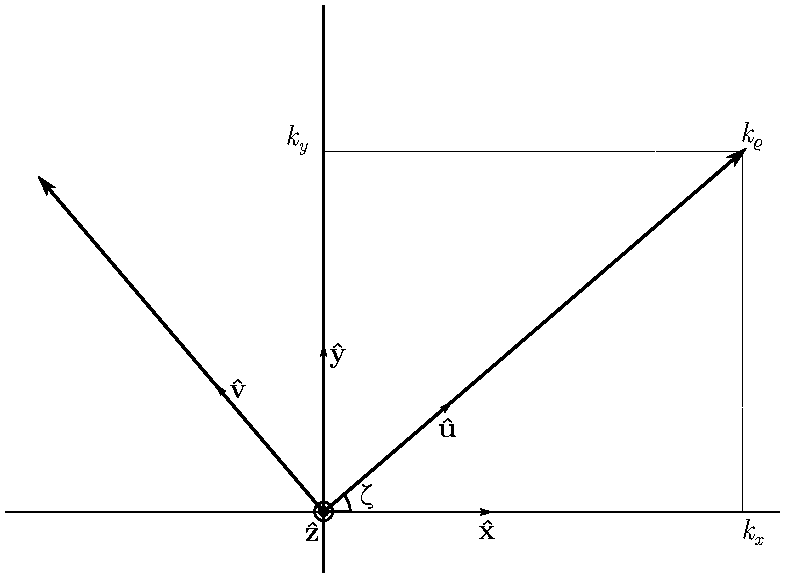
\includegraphics[scale=.75]{fig_coordinate.pdf}}
    \caption{Coordinate System in the spectral domain \cite[p. 1166]{michalski2005electromagnetic}}
    \label{fig:SpCS}
  \end{figure}

  \begin{equation}
    \left[\begin{array}{c}
    \v{\ti{E}_t} \\
    \v{\ti{H}_t}
    \end{array} \right]
    = \left[ \begin{array}{cc}
    V^e & V^h \\
    -I^h & I^e
    \end{array} \right]
    \left[\begin{array}{c}
    \v{\^u} \\
    \v{\^v}
    \end{array} \right]
    \label{eq:EHVI}
  \end{equation}
  where the superscripts e and h denote TM and TE mode respectively.
  %
  Using the results of (\ref{eq:EHVI}) in (\ref{eq:Et}) and noting that $\v{\^u} = \v{k_{\p}}/k_{\p}$, we get,
  \begin{equation}
    \dv{\left(\v{\^u}V^e + \v{\^v}V^h \right)}{z} = \frac{1}{j \O \E}\left( k^2 - \v{k_{\p}}\v{k_{\p}} \cdot \right) (\v{\^u} I^e + \v{\^v}I^h) + \v{\^u}k_{\p} \frac{\ti{J}_z}{\O \E} - (\v{\^u} \ti{M}_v - \v{\^v} \ti{M}_u)
    \label{eq:Vinuv}
  \end{equation}
  By separating the $\v{\^u}$ and $\v{\^v}$ components, we obtain the voltage equivalent TM and TE equations respectively.
  \begin{equation}
    \dv{V^e}{z} = \frac{1}{j \O \E}\left( k^2 - k_{\p}^2 \right)I^e + k_{\p}\frac{\ti{J}_z}{\O \E} - \ti{M}_v
    \label{eq:V_TM}
  \end{equation}
  \begin{equation}
    \dv{V^h}{z} = \frac{1}{j \O \E}k^2 I^h + \ti{M}_u
    \label{eq:V_TE}
  \end{equation}

  Similarly, from (\ref{eq:EHVI}) and (\ref{eq:Ht}), the current equivalent equations can be written as:
  \begin{equation}
    \dv{I^e}{z} = \frac{1}{j \O \u}k^2 V^e - \ti{J}_u
    \label{eq:I_TM}
  \end{equation}
  \begin{equation}
    \dv{I^h}{z} = \frac{-1}{j \O \u}\left( k^2 - k_{\p}^2 \right)V^h + k_{\p}\frac{\ti{M}_z}{\O \u} + \ti{J}_v
    \label{eq:I_TE}
  \end{equation}

  Equations (\ref{eq:V_TM}-\ref{eq:I_TE}) can be conveniently written collectively as a set of Telegrapher's equations \cite[p. 1166]{michalski2005electromagnetic}:
  \begin{subequations}
    \begin{align}
      \dv{V^{\alpha}}{z} ={}& -j k_z Z^{\alpha}I^{\alpha} + v^{\alpha}
      \label{eq:TL_V}\\
      \dv{I^{\alpha}}{z} ={}& -j k_z Y^{\alpha}V^{\alpha} + i^{\alpha}
      \label{eq:TL_I}
    \end{align}
    \label{eq:TLE}
  \end{subequations}
  where,
  \begin{equation}
    k_z = \sqrt{k^2 - k_{\p}^2}
    \label{eq:k_z}
  \end{equation}
  \begin{equation}
    \begin{split}
      Z^e = \frac{1}{Y^e} = \frac{k_z}{\O \E},\\
      Z^h = \frac{1}{Y^h} = \frac{\O \u}{k_z}\\
    \end{split}
    \label{eq:Z}
  \end{equation}

  From the preceding discussion, six source configurations, three each for electric and magnetic currents lead to a TM/TE based trasnmission line (TL). The type and strength of the TL excitation is determined from (\ref{eq:V_TM})-(\ref{eq:TLE}) and is summarized in Fig. \ref{fig:Sources}.

  \begin{figure}[t!]
    \centering
    {\includegraphics[scale=.6]{source_configuration.pdf}}
    \caption{Current Configuration and the respective TL equivalent}
    \label{fig:Sources}
  \end{figure}

  \bibliography{mylib}
  \bibliographystyle{ieeetr}

\end{document}
